\chapter{Analýza a srovnání}

\section{Vymezení fyziologické schopnosti}
Když se ptáme, proč se někdo dokázal něco naučit nebo naopak nedokázal, musíme se ptát, jestli byl schopný se to naučit.  V rámci studie, která se zabývá hmatem, musíme určit omezení hmatu.

Abych zajistil, že můj FCHAD je fyzicky použitelný, přečetl jsem si kapitolu \em Haptic Interfaces\em  v knize \em HCI Beyond the GUI\em. Člověk má šest druhů hmatových receptorů: volná nervová zakončení, Meissnerovo tělísko, Merkelovy buňky, Paciniho tělíska, receptory vlasového folikulu a Ruffiniho tělíska. Různé hmatové receptory mají různou citlivost.  Například Paciniho tělíska cítí jenom vibrace.

Pro účely FCHADu chceme spustit receptory, které reagují rychle a přesně.  Myslím si, že je také lepší spustit více druhů receptorů naráz, ale nejsem si jistý.  Prostorově nejpřesnější receptory jsou Meissnerova tělíska a Merkelovy buňky. Verze FCHADu použitá v hlavní studii produkuje malé vibrace o 200Hz, což je doporučená frekvence v publikace HCI \citep[str. 29-30]{nielsen2008gesture}.

Autoři citované kapitoly rozlišují čtyři subjektivní druhy hmatu: tlak, dotyk, vibrace a lechtání.  Myslím, že lechtání vzniká pohybem přes prsty.  Jedna z hypotéz, proč FCHADy nefungují moc dobře, říká, že čtenáři pomůže rozpoznat písmeno pohyb bodů na prstech.  Christophe Ramstein ve studii z roku 1996 píše o FCHADech: \em \uv{Protože se na hmatovém vnímání podílí více mechanických receptorů, pohyb prstů nad strukturou zlepšuje vnímání.  V případě jednoznakového zobrazovače prst necítí přechod mezi písmeny, ale jen změnu uspořádání.  Protože se prst nepohybuje, rychlost čtení je pomalejší než na zobrazovačích o 20ti, 40ti, anebo 80ti znacích (46.1 slov za minut u rychlého čtenáře a 12.0 slov za minutu u pomalého čtenáře)} \em  \citep[str. 38, přeloženo z angličtiny]{ramstein1996combining}
%"Because multiple mechanical receptors are involved in the tactile perception mechanism, the displacement of the finger over a form or texture improves perception and facilitates acknowledgement[7,14]. As a result, in the single cell case, the finger will not feel the transition from one character to the next, but only the configurational changes in the cell’s pins according to the following character.  Since the finger is not moving on the braille characters, speed performance will of course be slower than on 20-, 40- or 8O-cell braille displays (46.1 wpm for fast readers and 12.0 wpm for slow readers)."
Když čtu tištěné Braillovo písmo, pociťuji lechtání.  Abych podobný pocit zajistil u zobrazovače FCHADu, pokrývám ho kusem látky.  Mně osobně to tak vyhovuje, během studie jsem však látku nepoužíval. Domníval jsem se, že by pro účastníky mohla představovat komplikaci.

Publikace HCI sestavuje pro naše použití prahy rozlišení, v angličtině "Just Noticeable Differences (JND)". Na JND nepohlížím jako na měřítko toho, co člověk dokáže cítit, ale spíš toho, co nedokáže.  Nechtěl jsem, aby nástroj pracoval na hranici citlivosti, ale aby znaky byly bezpečně rozpoznatelné.

Pocit hmatu je přesný do ${}1mm^2 - 2mm^2$ na bříškách prstů a až ${}45mm^2$ jinde na těle.  Tištěné Braillovo písmo má body vzdálené od sebe 2.3-2.5mm \citep{brailleauthority}. To je až příliš blízko JND.  Perkins vyrábí speciální velkopísmenové psací stroje, protože někteří nevidomí nedokážou normální Braillovo písmo číst\footnote{\url{https://secure2.convio.net/psb/site/Ecommerce?FOLDER=1180&store_id=1101&JServSessionIdr004=9p1uhglug2.app246a&__utma=184864936.426189431.1365936556.1365946389.1366050996.3&__utmb=184864936.1.10.1366050996&__utmc=184864936&__utmx=-&__utmz=184864936.1365936556.1.1.utmcsr=(direct)|utmccn=(direct)|utmcmd=(none)&__utmv=-&__utmk=194396717}}.  Bohužel, když se písmo zvětší, už se nevejde na bříško prstu a kůže jinde na těle je méně citlivá.  Vzdálenost JND je na kůži na dlani 11mm a proto hrozí, že se zvětšením písma zhorší čtení. Můj osobní pocit je, že optimální velikost pro Braillovo písmo je 500 x 300mm.  Když jsem však vyráběl první FCHAD, nemohl jsem sehnat tak malé cívky, a proto jsem ve studii používal daleko větší zobrazovač, než bych si přál \citep[str. 30-32]{nielsen2008gesture}.

Další práh rozlišení je časový, který udává, kolikrát něco můžete cítit za sekundu.  V angličtině "successiveness limen(SL)" je minimální interval mezi dvěma impulzy, při kterém člověk impulzy od sebe rozliší. V naší studii žádný účastník nečetl tak rychle, aby se přiblížil SL.  Doufal jsem, že budou číst rychleji, a stále doufám, že bude možné na FCHADu číst tak rychle jako tištěné Braillovo písmo, což je asi 7.9 CPS \citep{wetzel2006studies}.  To znamená, že se za každých 126ms musí přečíst jedno písmeno.  SL pro mechanické receptory je 5 ms, ale nás zajímá 20 ms, což je minimální interval, při kterém člověk rozliší dva impulzy ve správném pořadí \citep[str. 32]{nielsen2008gesture}.

Dalším omezením je absolutní velikost ruky.  Pokud ruka není dost velká, nepokrývá celý zobrazovač.  Několik účastníků mělo ruce tak malé, že zobrazovač nepokryli dlaní pohodlně. Naštěstí se nenašel nikdo, kdo by toho nebyl schopný vůbec.

Na závěr bych řekl, že účastníci studie byli fyzicky schopní používat FCHAD správně a že hranice citlivosti nehrála ve studii roli.

\section{Analýza rychlosti}
Kdyby toto byla čistě psychologická studie, omezoval bych svoji vlastní přítomnost v zájmu srovnatelnosti výsledků.  Protože je to však pedagogický výzkum, jsem já jako pedagog a badatel neoddělitelnou součástí výsledků.

Nemůžeme v této studii nahlížet na rychlost čtení a křivky učení jako na absolutní hodnoty, protože rychlost čtení je ovlivněna do velké míry tím, jestli jsem já něco zdlouhavě vysvětloval nebo ne, a jestli jsem případné chyby opravil nebo ignoroval.

Kvůli velkým potížím se čtením je žák 8 z následující analýzy vynechán.

\paragraph{Jak číst grafy}  Grafy ukazují, který senzor byl v daném momentě vybrán.  Když nebyl vybrán žádný senzor, je to znázorněno stejným způsobem, jako když je vybrán senzor č.0.  Škála není normalizovaná. Číslo pod grafem je absolutní čas, tj. minuty dané hodiny, kdy studie probíhala.  Číslo 22m v grafu označeném 20-Mar-13 12:00 tedy znamená, že v daný moment bylo 12:22 (a NE tedy 22m od začátku experimentu, jak by se mohlo na první pohled zdát).  Když čára vypadá \uv{chlupatá}, znamená to, že byl špatný kontakt mezi prstem a senzorem.

Nemá smysl analyzovat časy čtení prvního řádku, protože jsem často účastníkům pomáhal a protože je kratší než ostatní.

% 3 = down 4 = up

\subsection{Žák 5}
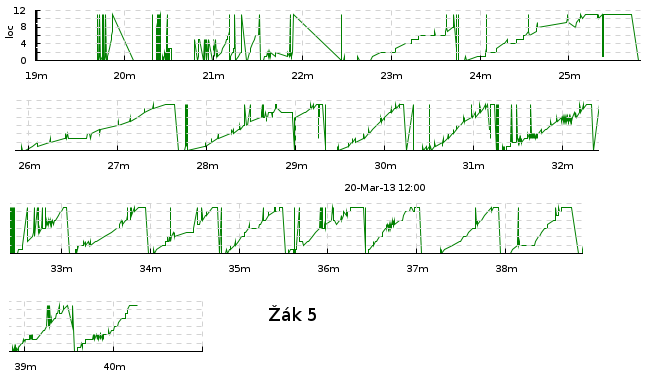
\includegraphics[width=1\textwidth]{Location5-cut}

Četl 17 řádků. Na grafu je 17 vrcholů, což odpovídá.

Dlouho jsem uvažoval, jak měřit rychlost čtení na FCHADu.  Sice mám hezké grafy, ale to neznamená, že mohu přesně měřit rychlost čtení.  Nezpracovaná data pro první tří písmena druhého řádku jsou (trojtečky značí, kde došlo ke změně dotýkaných senzorů, ale zobrazené písmeno se nezměnilo):
\begin{verbatim}
2013-03-20@12:23:44.436 Dolu  1 0 0 0 0 0 0 0 0 0 0 0 0 'k'
...
2013-03-20@12:23:49.634 Dolu  1 1 1 0 0 0 0 0 0 0 0 0 0 'k'
2013-03-20@12:23:49.964 Nahoru  0 1 1 0 0 0 0 0 0 0 0 0 1 'ý'
2013-03-20@12:23:50.129 Nahoru  0 1 0 0 0 0 0 0 0 0 0 0 1 'ý'
2013-03-20@12:23:50.212 Dolu  0 1 1 0 0 0 0 0 0 0 0 0 1 'ý'
2013-03-20@12:23:50.748 Dolu  1 1 1 0 0 0 0 0 0 0 0 0 0 'k'
2013-03-20@12:23:58.084 Nahoru 0 1 1 0 0 0 0 0 0 0 0 0 1 'ý'
2013-03-20@12:24:03.483 Dolu  0 1 1 1 0 0 0 0 0 0 0 0 1 'ý'
2013-03-20@12:24:03.525 Nahoru  0 0 1 1 0 0 0 0 0 0 0 0 2 ' '
...
2013-03-20@12:24:11.233 Dolu  0 0 1 1 1 0 0 0 0 0 0 0 2 ' '

\end{verbatim}

Nuly a jedničky značí, zda byl senzor aktivní. Například řádek
\begin{verbatim}
2013-03-20@12:24:11.233 Dolu  0 0 1 1 1 0 0 0 0 0 0 0 2 ' '
\end{verbatim}

znamená, že v 12:24:11.233 došlo k dotyku na třech senzorech a že se zobrazovala mezera.  Když se podíváte na čas 12:23:50.212, začíná se zobrazovat `ý', ale v 12:23:50.748 se vrací `k'.  Není z toho jasné, kdy čtení jednoho písmene končí a kdy čtení dalšího začíná.  Všechna shromážděná data jsou takto nejasná.  Proto jsem si vybral způsob analýzy očima za pomoci kružítka.

Pátý žák se během našeho setkání značně zrychlil.

Prvních pět řádků se zrychloval každým řádkem, ale mezi pátým řádkem a šestým řádkem není rozdíl v rychlosti. Sedmý řádek četl zase pomaleji, ale osmý řádek byl jeho nejrychlejší řádek vůbec. Devátý řádek zase četl stejně rychle jako pátý.  Na desátém řádku zpomalil.  Zbytek času zrychloval nebo zpomaloval bez rozpoznatelné tendence.

Nelze přesně měřit čas čtení na FCHADu, ale mohl jsem měřit čas od chvíle, kdy žák poprvé umístil ruku na selektor, do chvíle, kdy ji naposledy stáhl. Žák 5 četl na FCHADu jenom 17:02 minut a za tu dobu přečetl 196 znaků.  To je přibližně 0.2 znaků za sekundu. Když to srovnáme s jeho rychlostí čtení tištěného textu (11.37 CPS), vidíme, že na FCHADu během našeho setkání četl až 60krát pomaleji.

\subsection{Žák 6}
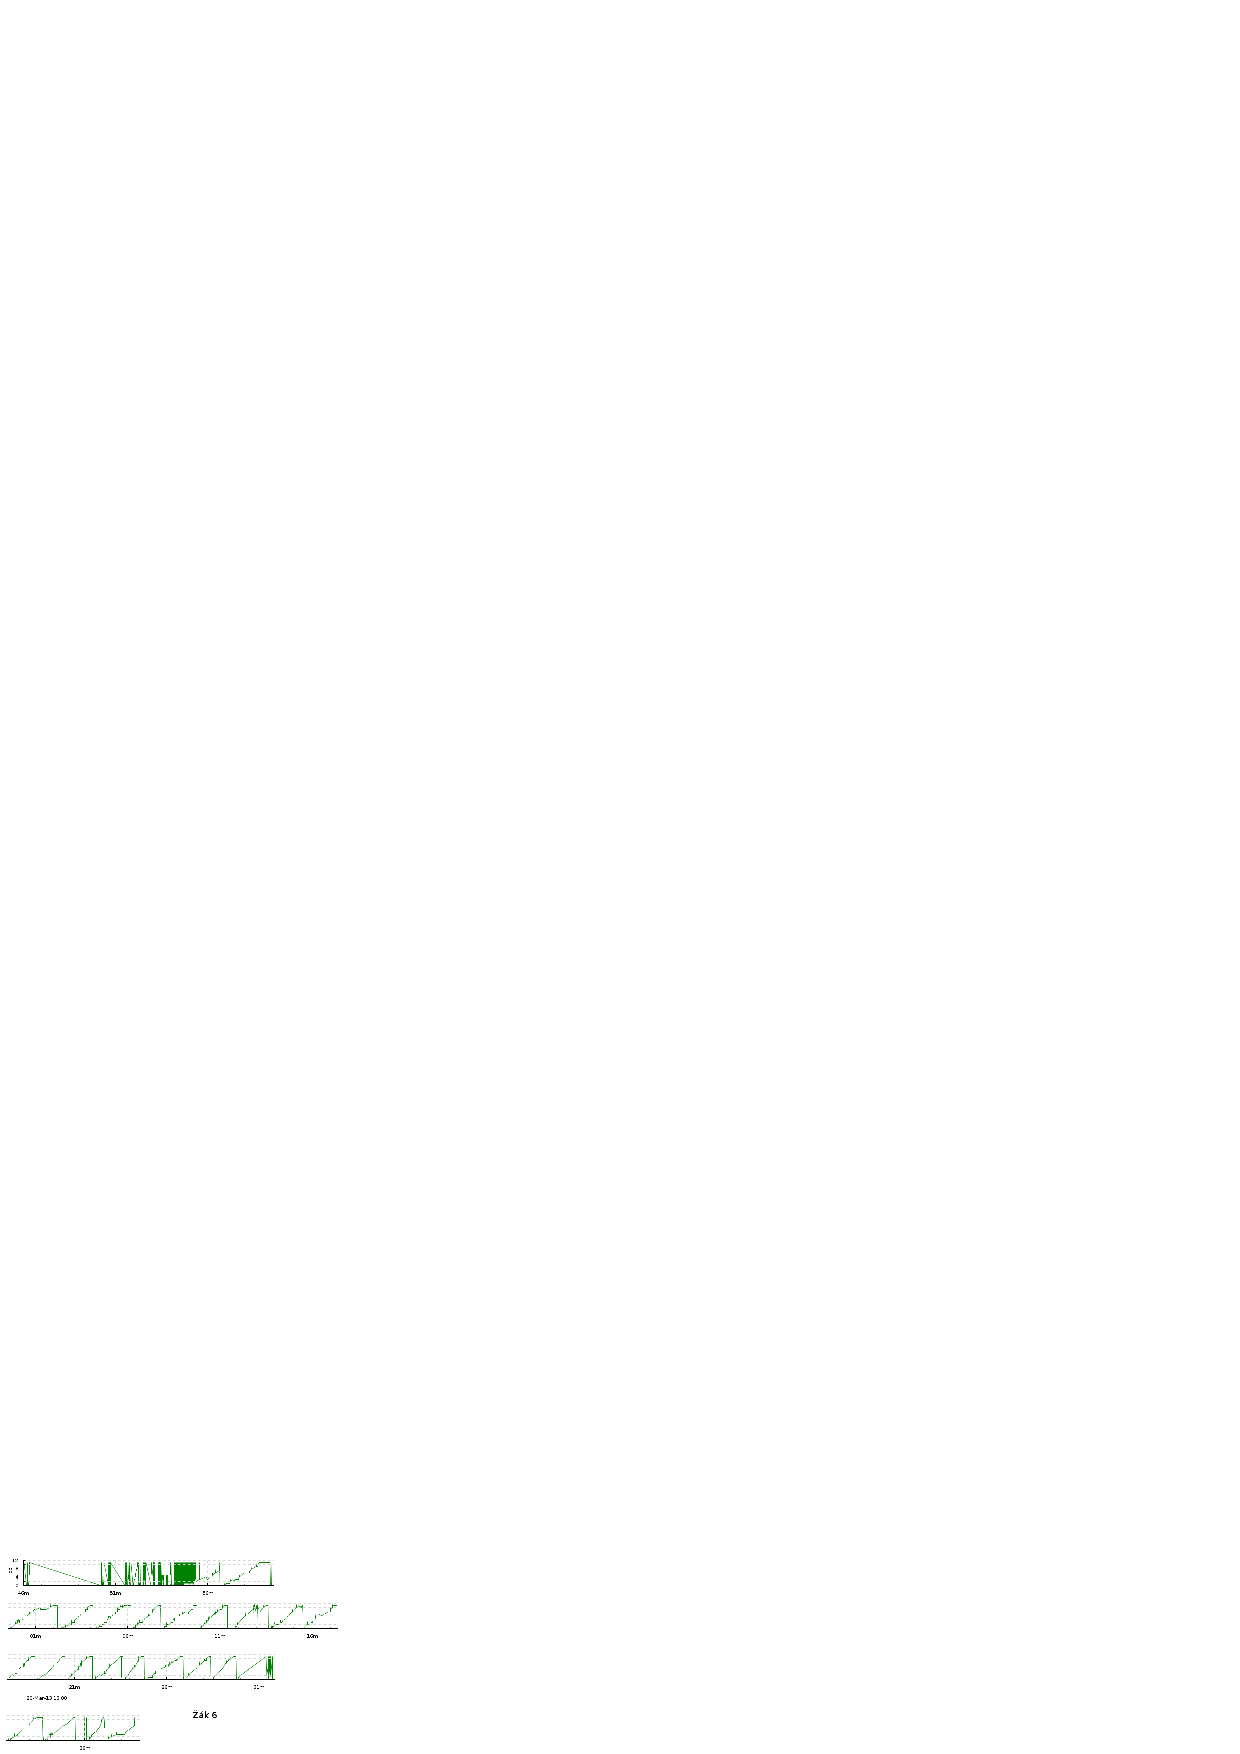
\includegraphics[width=1\textwidth]{Location6-cut}

Četla 22 řádků, přičemž z posledního jenom prvních 7 znaků.  Na grafu je 24 vrcholů: Vrchol s rovnou čárou kolem 31m není čtení (pouze přejetí prstem po senzorech) a předposlední řádek četla dvakrát.

Žákyně 6 se také zrychlila, ale ne tak pravidelně jako žák 5.

Druhý a třetí řádek četla stejně rychle.  Čtvrtý řádek četla rychleji, ale u pátého řádku trochu zpomalila. Dále nebyla tendence rozeznatelná.  Mezi řádky 12 a 16 se pomalu zrychlovala, ale na řádku 17 opět značně zpomalila.  Dále nelze rozeznat tendenci.  Předposlední řádek, kdy měla číst slova a ne písmena, a který četla podruhé, četla značně rychleji.

Žákyně 6 přečetla na FCHADu 249 znaků během 44:42 minut.  To je kolem 0.09 znaků za sekundu. Když to srovnáme s její rychlostí čtení tištěného textu (6.7 CPS), vidíme, že na FCHADu četla během našeho setkání až 72krát pomaleji.


\subsection{Žák 7}
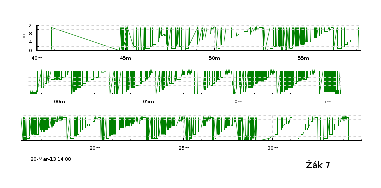
\includegraphics[width=1\textwidth]{Location7-cut}

Četl 19 řádků. Desátý řádek četl dvakrát, proto je na grafu dvacet vrcholů.

První čtyři řádky četl stejnou rychlostí. Během čtení pátého řádku odstranil prst ze selektoru, proto je vrchol na grafu rozdělený. Šestý řádek četl rychleji než ty první, ale pak se jeho rychlost nezměnila až do třináctého řádku, kdy zase zrychlil.  Čtrnáctý řádek je pomalý, ale zbytek doby zrychloval.


Žák 7 přečetl na FCHADu 215 znaků během 48:48 minut.  To je kolem 0.07 znaků za sekundu. Když to srovnáme s jeho rychlostí čtení tištěného textu (8.24 CPS), vidíme, že na FCHADu četl během našeho setkání až 112krát pomaleji.

\subsection{Žák 9}
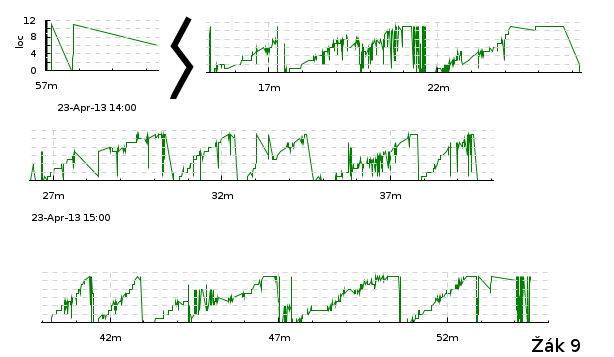
\includegraphics[width=1\textwidth]{Location9-cut}

Četl 13 řádků, na grafu je 13 vrcholů.

První čtyři řádky četl stejnou rychlostí, pátý řádek byl rychlejší a šestý stejně rychlý jako pátý. Sedmý je pomalý, ale na osmém až desátém zrychloval.  Velké zpomalení je vidět u jedenáctého řádku, snad proto, že jsou tam čísla. A poslední dva řádky jsou pomalé, protože používal selektor samostatně.

Žák 9 přečetl na FCHADu 148 znaků během 39:12 minut.  To je kolem 0.06 znaků za sekundu. Když to srovnáme s jeho rychlostí čtení tištěného textu (5 CPS), vidíme, že na FCHADu četl během našeho setkání až 79krát pomaleji.

Je jasné, že pokud jde o rychlost, je co zlepšovat.

\subsection{Analýza chyb}

Zde uvádím shromážděné chyby účastníků hlavní studie.  Opět vynechávám výsledky účastníka 8.

\begin{tabular}{|c|c|}
\hline
Symbol&Význam\\
\hline
NČ&Nečetl samostatně\\
\hline
??&Chyba, ale na nahrávce nebylo poznat jaká\\
\hline
>>&Přeskočil písmeno\\
\hline
*&Na nahrávce není poznat, zda udělal chybu\\
\hline
ZVP&Znak pro velká písmena\\
\hline
--&Četl s pomocí\\
\hline
\end{tabular}


%\paragraph{První Řádek}
\begin{tabular}{|c|c|c|c|c|c|c|c|c|c|c|c|c|}
\hline
Žák&B&r&a&i&l&l&s&&&&&\\
&\braillebox{1278}&\braillebox{1235}&\braillebox{1}&\braillebox{24}&\braillebox{123}&\braillebox{123}&\braillebox{234}&\braillebox{}&\braillebox{2358}&\braillebox{123}&\braillebox{}&\braillebox{}\\
\hline
5&&NČ&NČ&s&&&&>>&>>&>>&>>&>>\\
&&&&\braillebox{234}&&&&&&&&\\
\hline
6&v&&&&??&&&>>&>>&>>&>>&>>\\
&\braillebox{1236}&&&&&&&&&&&\\
\hline
7&ě&h&&,&&>>&&>>&>>&>>&>>&>>\\
&\braillebox{126}&\braillebox{125}&&\braillebox{2}&&&&&&&&\\
\hline
9&NČ&--&&&&&p&>>&>>&>>&>>&>>\\
&&&&&&&\braillebox{1234}&&&&&\\
\hline
\end{tabular}

%\paragraph{Druhý Řádek}
\begin{tabular}{|c|c|c|c|c|c|c|c|c|c|c|c|c|}
\hline
Žák&k&ý& &ř&á&d&e&k&,& &k&t\\
&\braillebox{1378}&\braillebox{12346}&\braillebox{}&\braillebox{2456}&\braillebox{16}&\braillebox{145}&\braillebox{15}&\braillebox{13}&\braillebox{2}&\braillebox{}&\braillebox{13}&\braillebox{2345}\\
\hline
5&&&&&&&&&NČ&&&\\
\hline
6&a&?p?&&?t?&&&??&&NČ&&&j\\
&\braillebox{1}&\braillebox{1234}&&\braillebox{2345}&&&&&&&&\braillebox{245}\\
\hline
7&&&&&&&&&&&&\\
\hline
9&&&&&&&&&&&a&\\
&&&&&&&&&&&\braillebox{1}&\\
\hline
\end{tabular}

%\paragraph{Třetí Řádek}
\begin{tabular}{|c|c|c|c|c|c|c|c|c|c|c|c|c|}
\hline
Žák&e&r&ý& &t&e&ď& &p&o&u&ž\\
&\braillebox{1578}&\braillebox{1235}&\braillebox{12346}&\braillebox{}&\braillebox{2345}&\braillebox{15}&\braillebox{1456}&\braillebox{}&\braillebox{1234}&\braillebox{135}&\braillebox{136}&\braillebox{2346}\\
\hline
5&&&&&&??&&&&&&\\
\hline
6&&&&&&&&&&r&&\\
&&&&&&&&&&\braillebox{1235}&&\\
\hline
7&&&&&&o&&&&k&&\\
&&&&&&\braillebox{135}&&&&\braillebox{13}&&\\
\hline
9&&&&&&&&&&&&z\\
&&&&&&&&&&&&\braillebox{1356}\\
\hline
\end{tabular}

%\paragraph{Čtvrtý Řádek}
\begin{tabular}{|c|c|c|c|c|c|c|c|c|c|c|c|c|}
\hline
Žák&í&v&á&t&e&,& &n&e&n&í& \\
&\braillebox{3478}&\braillebox{1236}&\braillebox{16}&\braillebox{2345}&\braillebox{15}&\braillebox{2}&\braillebox{}&\braillebox{1345}&\braillebox{15}&\braillebox{1345}&\braillebox{34}&\braillebox{}\\
\hline
5&&&&j&&&&d&&&&\\
&&&&\braillebox{245}&&&&\braillebox{145}&&&&\\
\hline
6&&l&&&&&&&&&&\\
&&\braillebox{123}&&&&&&&&&&\\
\hline
7&&&u&&o&&&d&&&&\\
&&&\braillebox{136}&&\braillebox{135}&&&\braillebox{145}&&&&\\
\hline
9&á&&&&i&&&ž(NČ)&>>&>>&t,á&\\
&\braillebox{16}&&&&\braillebox{24}&&&\braillebox{2346}&&&\braillebox{2345},\braillebox{16}&\\
\hline
\end{tabular}

%\paragraph{Pátý Řádek}
\begin{tabular}{|c|c|c|c|c|c|c|c|c|c|c|c|c|}
\hline
Žák&p&r&v&n&í& &ř&á&d&e&k&,\\
&\braillebox{123478}&\braillebox{1235}&\braillebox{1236}&\braillebox{1345}&\braillebox{34}&\braillebox{}&\braillebox{1235}&\braillebox{16}&\braillebox{145}&\braillebox{15}&\braillebox{13}&\braillebox{2}\\
\hline
5&&&&&&&&&&&&\\
\hline
6&&&&&&&&&&&a&NČ\\
&&&&&&&&&&&\braillebox{1}&\\
\hline
7&&&&&&*&*&*&*&*&*&*\\
\hline
9&&&&&&&&í&&&a&\\
&&&&&&&&\braillebox{34}&&&\braillebox{1}&\\
\hline
\end{tabular}

%\paragraph{Šestý Řádek}
\begin{tabular}{|c|c|c|c|c|c|c|c|c|c|c|c|c|}
\hline
Žák& &k&t&e&r&ý& &z&o&b&r&a\\
&\braillebox{78}&\braillebox{13}&\braillebox{2345}&\braillebox{15}&\braillebox{1235}&\braillebox{12346}&\braillebox{}&\braillebox{1356}&\braillebox{135}&\braillebox{12}&\braillebox{1235}&\braillebox{1}\\
\hline
5&&&&&&&&&&&&\\
\hline
6&&&&&&&&&&&&\\
\hline
7&&&&&&&&ř&&&&\\
&&&&&&&&\braillebox{2456}&&&&\\
\hline
9&&&&&&&&n&&&h&\\
&&&&&&&&\braillebox{1345}&&&\braillebox{125}&\\
\hline
\end{tabular}

%\paragraph{Řádek 7}
\begin{tabular}{|c|c|c|c|c|c|c|c|c|c|c|c|c|}
\hline
Žák&z&u&j&e& &j&e&n&o&m& &j\\
&\braillebox{135678}&\braillebox{136}&\braillebox{245}&\braillebox{15}&\braillebox{}&\braillebox{245}&\braillebox{15}&\braillebox{1345}&\braillebox{135}&\braillebox{134}&\braillebox{}&\braillebox{245}\\
\hline
5&&&&&&&&&&&&\\
\hline
6&&&&&&&&d&&&&\\
&&&&&&&&\braillebox{145}&&&&\\
\hline
7&&&&&&&&&&&&\\
\hline
9&n&a&h&&&h&&d&&k&&,\\
&\braillebox{1345}&\braillebox{1}&\braillebox{125}&&&\braillebox{125}&&\braillebox{145}&&\braillebox{13}&&\braillebox{2}\\
\hline
\end{tabular}

%\paragraph{Řádek 8}
\begin{tabular}{|c|c|c|c|c|c|c|c|c|c|c|c|c|}
\hline
Žák&e&d&n&o& &p&í&s&m&e&n&o\\
&\braillebox{1578}&\braillebox{145}&\braillebox{1345}&\braillebox{135}&\braillebox{}&\braillebox{1234}&\braillebox{34}&\braillebox{234}&\braillebox{134}&\braillebox{15}&\braillebox{1345}&\braillebox{135}\\
\hline
5&&&&&&&&&&&&\\
\hline
6&&&&&&&&&&&&\\
\hline
7&&&&&&&&??&&&&a\\
&&&&&&&&&&&&\braillebox{1}\\
\hline
9&&&&&&&á&&c&o&&e\\
&&&&&&&\braillebox{16}&&\braillebox{14}&\braillebox{135}&&\braillebox{15}\\
\hline
\end{tabular}

%\paragraph{Řádek 9}
\begin{tabular}{|c|c|c|c|c|c|c|c|c|c|c|c|c|}
\hline
Žák&.& & &P&r&v&n&í& &b&y&l\\
&\braillebox{378}&\braillebox{}&\braillebox{}&\braillebox{12347}&\braillebox{1235}&\braillebox{1236}&\braillebox{1345}&\braillebox{34}&\braillebox{}&\braillebox{12}&\braillebox{13456}&\braillebox{123}\\
\hline
5&&&&&&&&&&&&\\
\hline
6&NČ&&&&&&&&&&&\\
\hline
7&&&&&&&&&&&&\\
\hline
9&(,ZVP&&&&&&&&&&&\\
&\braillebox{236},\braillebox{6}&&&&&&&&&&&\\
\hline
\end{tabular}

%\paragraph{Řádek 10}
\begin{tabular}{|c|c|c|c|c|c|c|c|c|c|c|c|c|}
\hline
Žák& &v&y&n&a&l&e&z&e&n& &v\\
&\braillebox{78}&\braillebox{1236}&\braillebox{13456}&\braillebox{1345}&\braillebox{1}&\braillebox{123}&\braillebox{15}&\braillebox{1356}&\braillebox{15}&\braillebox{1345}&\braillebox{}&\braillebox{1236}\\
\hline
5&&&&&&&&&&&&\\
\hline
6&&&?ď ?&&&&&&&&&\\
&&&\braillebox{1456}&&&&&&&&&\\
\hline
7&&??&&&&&o&&&&&\\
&&&&&&&\braillebox{135}&&&&&\\
\hline
9&&&&&&b&&&&&&\\
&&&&&&\braillebox{12}&&&&&&\\
\hline
\end{tabular}

%\paragraph{Řádek 11}
\begin{tabular}{|c|c|c|c|c|c|c|c|c|c|c|c|c|}
\hline
Žák& &r&o&c&e& &1&9&1&3& &v\\
&\braillebox{78}&\braillebox{1235}&\braillebox{135}&\braillebox{14}&\braillebox{15}&\braillebox{}&\braillebox{18}&\braillebox{248}&\braillebox{18}&\braillebox{148}&\braillebox{}&\braillebox{1236}\\
\hline
5&&&&&&&&&&&&\\
\hline
6&&&&&&&a&i&&&&\\
&&&&&&&\braillebox{1}&\braillebox{24}&&&&\\
\hline
7&&&&n&&&a&i&&&&l,r\\
&&&&\braillebox{1345}&&&\braillebox{1}&\braillebox{24}&&&&\braillebox{123},\braillebox{1235}\\
\hline
9&&ř&e,a&&&&a&i&&&&\\
&&\braillebox{2456}&\braillebox{15},\braillebox{1}&&&&\braillebox{1}&\braillebox{24}&&&&\\
\hline
\end{tabular}

%\paragraph{Řádek 12}
\begin{tabular}{|c|c|c|c|c|c|c|c|c|c|c|c|c|}
\hline
Žák& &A&n&g&l&i&i&.& & &J&m\\
&\braillebox{78}&\braillebox{17}&\braillebox{1345}&\braillebox{1245}&\braillebox{123}&\braillebox{24}&\braillebox{24}&\braillebox{3}&\braillebox{}&\braillebox{}&\braillebox{2457}&\braillebox{134}\\
\hline
5&&&d&&&&&mezera&&&&\\
&&&\braillebox{145}&&&&&\braillebox{}&&&&\\
\hline
6&&&&&&&9&&&&--&\\
&&&&&&&\braillebox{248}&&&&&\\
\hline
7&&&&&&e&&&&&&\\
&&&&&&\braillebox{15}&&&&&&\\
\hline
9&&&d&x&b&&&&&&,&c\\
&&&\braillebox{145}&\braillebox{1346}&\braillebox{12}&&&&&&\braillebox{2}&\braillebox{14}\\
\hline
\end{tabular}

%\paragraph{Řádek 13}
\begin{tabular}{|c|c|c|c|c|c|c|c|c|c|c|c|c|}
\hline
Žák&e&n&o&v&a&l& &s&e& &O&p\\
&\braillebox{1578}&\braillebox{1345}&\braillebox{135}&\braillebox{1236}&\braillebox{1}&\braillebox{123}&\braillebox{}&\braillebox{234}&\braillebox{15}&\braillebox{}&\braillebox{1357}&\braillebox{1234}\\
\hline
5&&&&&&&&&&&n&\\
&&&&&&&&&&&\braillebox{1345}&\\
\hline
6&*&*&r&&&&&&&&&\\
&&&\braillebox{1235}&&&&&&&&&\\
\hline
7&&&&l&&&&&&&&\\
&&&&\braillebox{123}&&&&&&&&\\
\hline
9&&&e&&&&&&&&k&l\\
&&&\braillebox{15}&&&&&&&&\braillebox{13}&\braillebox{123}\\
\hline
\end{tabular}

%\paragraph{Řádek 14}
\begin{tabular}{|c|c|c|c|c|c|c|c|c|c|c|c|c|}
\hline
Žák&t&o&f&o&n& &a& &p&ř&e&v\\
&\braillebox{234578}&\braillebox{135}&\braillebox{124}&\braillebox{135}&\braillebox{1345}&\braillebox{}&\braillebox{1}&\braillebox{}&\braillebox{1234}&\braillebox{2456}&\braillebox{15}&\braillebox{1236}\\
\hline
5&&&&&&&&&&&&\\
\hline
6&j&&&&&&&&n&&&\\
&\braillebox{245}&&&&&&&&\braillebox{1345}&&&\\
\hline
7&&&&&&&&&&&&\\
\hline
\end{tabular}

%\paragraph{Řádek 15}
\begin{tabular}{|c|c|c|c|c|c|c|c|c|c|c|c|c|}
\hline
Žák&á&d&ě&l& &s&v&ě&t&l&o& \\
&\braillebox{1678}&\braillebox{145}&\braillebox{126}&\braillebox{123}&\braillebox{}&\braillebox{234}&\braillebox{1236}&\braillebox{126}&\braillebox{2345}&\braillebox{123}&\braillebox{135}&\braillebox{}\\
\hline
5&&&&&&&&&&&&\\
\hline
6&&&v&&&i&&&j&&&\\
&&&\braillebox{1236}&&&\braillebox{15}&&&\braillebox{245}&&&\\
\hline
7&&&&&&&&&&&&\\
\hline
\end{tabular}

%\paragraph{Řádek 16}
\begin{tabular}{|c|c|c|c|c|c|c|c|c|c|c|c|c|}
\hline
Žák&n&a& &z&v&u&k&.& & &K&d\\
&\braillebox{134578}&\braillebox{1}&\braillebox{}&\braillebox{1356}&\braillebox{1236}&\braillebox{136}&\braillebox{13}&\braillebox{3}&\braillebox{}&\braillebox{}&\braillebox{137}&\braillebox{145}\\
\hline
5&&&&e&&&&&&&&\\
&&&&\braillebox{15}&&&&&&&&\\
\hline
6&&&&&&&&&&&&\\
\hline
7&&&&&&&&&&&&\\
\hline
\end{tabular}

%\paragraph{Řádek 17}
\begin{tabular}{|c|c|c|c|c|c|c|c|c|c|c|c|c|}
\hline
Žák&y&ž& &č&t&e&n&á&ř& &p&o\\
&\braillebox{1345678}&\braillebox{2346}&\braillebox{}&\braillebox{146}&\braillebox{2345}&\braillebox{15}&\braillebox{1345}&\braillebox{16}&\braillebox{2456}&\braillebox{}&\braillebox{1234}&\braillebox{135}\\
\hline
5&&&&&&&&&&&&\\
\hline
6&&&&&j&&k&&&&&\\
&&&&&\braillebox{245}&&\braillebox{13}&&&&&\\
\hline
7&ď&&&??&&&&&&&&\\
&\braillebox{1456}&&&&&&&&&&&\\
\hline
\end{tabular}

%\paragraph{Řádek 18}
\begin{tabular}{|c|c|c|c|c|c|c|c|c|c|c|c|c|}
\hline
Žák&h&y&b&o&v&a&l& &s&p&e&c\\
&\braillebox{12578}&\braillebox{13456}&\braillebox{12}&\braillebox{135}&\braillebox{1236}&\braillebox{1}&\braillebox{123}&\braillebox{}&\braillebox{234}&\braillebox{1234}&\braillebox{15}&\braillebox{14}\\
\hline
6&&&&&&&&&&&&\\
\hline
7&??&d&&&&&&&&&&\\
&&\braillebox{145}&&&&&&&&&&\\
\hline
\end{tabular}

%\paragraph{Řádek 19}
\begin{tabular}{|c|c|c|c|c|c|c|c|c|c|c|c|c|}
\hline
Žák&i&á&l&n&í&m& &p&e&r&e&m\\
&\braillebox{2478}&\braillebox{16}&\braillebox{123}&\braillebox{1345}&\braillebox{34}&\braillebox{134}&\braillebox{}&\braillebox{1234}&\braillebox{15}&\braillebox{1235}&\braillebox{15}&\braillebox{134}\\
\hline
6&&&&&&&&&&&&\\
\hline
7&s&e&&&&&&&o&&&p\\
&\braillebox{234}&\braillebox{15}&&&&&&&\braillebox{135}&&&\braillebox{1234}\\
\hline
\end{tabular}

%\paragraph{Řádek 20}
\begin{tabular}{|c|c|c|c|c|c|c|c|c|c|c|c|c|}
\hline
Žák& &n&a&d& &p&í&s&m&e&n&e\\
&\braillebox{78}&\braillebox{1345}&\braillebox{1}&\braillebox{145}&\braillebox{}&\braillebox{1234}&\braillebox{34}&\braillebox{234}&\braillebox{134}&\braillebox{15}&\braillebox{1345}&\braillebox{15}\\
\hline
6&&&&&&&&&&&&\\
\hline
\end{tabular}

%\paragraph{Řádek 21}
\begin{tabular}{|c|c|c|c|c|c|c|c|c|c|c|c|c|}
\hline
Žák&m&,& &p&ř&í&s&t&r&o&j& \\
&\braillebox{13478}&\braillebox{2}&\braillebox{}&\braillebox{1234}&\braillebox{2456}&\braillebox{34}&\braillebox{234}&\braillebox{2345}&\braillebox{1235}&\braillebox{135}&\braillebox{245}&\braillebox{}\\
\hline
6&&&&&&&&&&&&\\
\hline
\end{tabular}

%\paragraph{Řádek 22}
\begin{tabular}{|c|c|c|c|c|c|c|c|c|c|c|c|c|}
\hline
Žák&b&z&u&č&e&l&.& & &T&o& \\
&\braillebox{1278}&\braillebox{1356}&\braillebox{136}&\braillebox{146}&\braillebox{15}&\braillebox{123}&\braillebox{3}&\braillebox{}&\braillebox{}&\braillebox{23457}&\braillebox{135}&\braillebox{}\\
\hline
6&&&&&&&&>>&>>&>>&>>&>>\\
\hline
\end{tabular}
\clearpage
\begin{figure}
\subsection{Druhy chyb}
\begin{subfigure}{.5\textwidth}
\centering
Zrcadlení - převážně u žáka 9

\begin{tabular}{|c|c|c|}
\hline
Počet&Správné písmeno&Chybné písmeno\\
\hline
1&ž\braillebox{2346}&z\braillebox{1356}\\
\hline
1&í\braillebox{3478}&á\braillebox{16}\\
\hline
2&í\braillebox{34}&á\braillebox{16}\\
\hline
1&e\braillebox{15}&i\braillebox{24}\\
\hline
1&i\braillebox{24}&e\braillebox{15}\\
\hline
1&n\braillebox{1345}&ž\braillebox{2346}\\
\hline
1&z\braillebox{1356}&n\braillebox{1345}\\
\hline
1&z\braillebox{135678}&n\braillebox{1345}\\
\hline
2&j\braillebox{245}&h\braillebox{125}\\
\hline
1&.\braillebox{378}&ZVP\braillebox{6}\\
\hline
1&r\braillebox{1235}&ř\braillebox{2456}\\
\hline
14\\
\hline
\end{tabular}
\end{subfigure}
\begin{subfigure}{.5\textwidth}
\centering
Nečetl dolní bod

\begin{tabular}{|c|c|c|}
\hline
Počet&Správné\newline písmeno&Chybné písmeno\\
\hline
2&r\braillebox{1235}&h\braillebox{125}\\
\hline
1&k\braillebox{1378}&a\braillebox{1}\\
\hline
3&k\braillebox{13}&a\braillebox{1}\\
\hline
1&ý\braillebox{12346}&p\braillebox{1234}\\
\hline
4&t\braillebox{2345}&j\braillebox{245}\\
\hline
1&t\braillebox{234578}&j\braillebox{245}\\
\hline
6&n\braillebox{1345}&d\braillebox{145}\\
\hline
1&u\braillebox{136}&a\braillebox{1}\\
\hline
2&m\braillebox{134}&c\braillebox{14}\\
\hline
3&o\braillebox{135}&e\braillebox{15}\\
\hline
2&l\braillebox{123}&b\braillebox{12}\\
\hline
1&y\braillebox{13456}&ď\braillebox{1456}\\
\hline
1&y\braillebox{1345678}&ď\braillebox{1456}\\
\hline
1&y\braillebox{1345678}&d\braillebox{145}\\
\hline
1&z\braillebox{1356}&e\braillebox{15}\\
\hline
30\\
\hline
\end{tabular}
\end{subfigure}

\begin{subfigure}{1\textwidth}
\centering
Body sedm a osm je mátly

\begin{tabular}{|c|c|c|}
\hline
Počet&Správné písmeno&Chybné písmeno\\
\hline
1&B\braillebox{1278}&v\braillebox{1236}\\
\hline
1&B\braillebox{1278}&ě\braillebox{126}\\
\hline
3&1\braillebox{18}&a\braillebox{1}\\
\hline
1&i\braillebox{24}&9\braillebox{248}\\
\hline
3&9\braillebox{248}&i\braillebox{24}\\
\hline
9\\
\hline
\end{tabular}
\end{subfigure}
\end{figure}
\begin{figure}
\begin{subfigure}{.5\textwidth}
\centering
Nečetli pravý sloupec bodů

\begin{tabular}{|c|c|c|}
\hline
Počet&Správné písmeno&Chybné písmeno\\
\hline
1&i\braillebox{24}&,\braillebox{2}\\
\hline
1&o\braillebox{135}&k\braillebox{13}\\
\hline
1&v\braillebox{1236}&l\braillebox{123}\\
\hline
1&m\braillebox{134}&k\braillebox{13}\\
\hline
2&j\braillebox{245}&,\braillebox{2}\\
\hline
2&v\braillebox{1236}&l\braillebox{123}\\
\hline
1&O\braillebox{1357}&k\braillebox{13}\\
\hline
1&p\braillebox{1234}&l\braillebox{123}\\
\hline
1&n\braillebox{1345}&k\braillebox{13}\\
\hline
11\\
\hline
\end{tabular}
\end{subfigure}
\begin{subfigure}{.5\textwidth}
\centering
Přidali nějaký bod

\begin{tabular}{|c|c|c|}
\hline
Počet&Správné písmeno&Chybné písmeno\\
\hline
2&i\braillebox{24}&s\braillebox{234}\\
\hline
1&s\braillebox{23478}&i\braillebox{15}\\
\hline
1&s\braillebox{234}&p\braillebox{1234}\\
\hline
5&e\braillebox{15}&o\braillebox{135}\\
\hline
2&o\braillebox{135}&r\braillebox{1235}\\
\hline
1&á\braillebox{16}&u\braillebox{136}\\
\hline
1&ě\braillebox{126}&v\braillebox{1236}\\
\hline
1&m\braillebox{134}&p\braillebox{1234}\\
\hline
14\\
\hline
\end{tabular}
\end{subfigure}
\begin{subfigure}{1\textwidth}
\centering
Nemám vysvětlení / Jiné

\begin{tabular}{|c|c|c|}
\hline
Počet&Správné písmeno&Chybné písmeno\\
\hline
1&ř\braillebox{2456}&t\braillebox{2345}\\
\hline
1&í\braillebox{34}&t\braillebox{2345}\\
\hline
1&z\braillebox{1345}&ř\braillebox{2456}\\
\hline
1&.\braillebox{378}&(\braillebox{236}\\
\hline
1&c\braillebox{14}&n\braillebox{1345}\\
\hline
1&v\braillebox{1236}&r\braillebox{1235}\\
\hline
1&g\braillebox{1245}&x\braillebox{1346}\\
\hline
1&O\braillebox{1357}&n\braillebox{1345}\\
\hline
1&p\braillebox{1234}&n\braillebox{1345}\\
\hline
1&á\braillebox{16}&e\braillebox{15}\\
\hline
10\\
\hline
\end{tabular}
\end{subfigure}
\end{figure}

\clearpage
\subsection{Počty chyb}
Žák 5 udělal 8 chyb na 196 přečtených znaků: jedna chyba na 24.5 znaků.

Žákyně 6 udělala 24 chyb na 249 přečtených znaků: jedna chyba na 10.375 znaků.

Žák 7 udělal 27 chyb na 215 přečtených znaků: jedna chyba na 7.963\_{} znaků

Žák 9 udělal 37 chyb na 148 přečtených znaků: jedna chyba na 4 znaky

Zde je tabulka počtů chyb na znak:

\begin{tabular}[hb]{|c|c|c|c|c|}
\hline
Řádek&Žák 5&Žák 6&Žák 7&Žák 9\\
\hline
1&$\frac{1}{5}$&$\frac{2}{7}$&$\frac{3}{6}$&$\frac{1}{6}$\\
\hline
2&$\frac{0}{12}$&$\frac{5}{11}$&$\frac{0}{12}$&$\frac{1}{12}$\\
\hline
3&$\frac{1}{12}$&$\frac{1}{12}$&$\frac{2}{12}$&$\frac{1}{12}$\\
\hline
4&$\frac{2}{12}$&$\frac{1}{12}$&$\frac{3}{12}$&$\frac{4}{10}$\\
\hline
5&$\frac{0}{12}$&$\frac{1}{11}$&$\frac{0}{5}$&$\frac{2}{12}$\\
\hline
6&$\frac{0}{12}$&$\frac{0}{12}$&$\frac{1}{12}$&$\frac{2}{12}$\\
\hline
7&$\frac{0}{12}$&$\frac{1}{12}$&$\frac{0}{12}$&$\frac{7}{12}$\\
\hline
8&$\frac{0}{12}$&$\frac{0}{12}$&$\frac{2}{12}$&$\frac{4}{12}$\\
\hline
9&$\frac{0}{12}$&$\frac{0}{11}$&$\frac{0}{12}$&$\frac{1}{12}$\\
\hline
10&$\frac{0}{12}$&$\frac{1}{12}$&$\frac{2}{12}$&$\frac{1}{12}$\\
\hline
11&$\frac{0}{12}$&$\frac{2}{12}$&$\frac{4}{12}$&$\frac{4}{12}$\\
\hline
12&$\frac{2}{12}$&$\frac{2}{12}$&$\frac{1}{12}$&$\frac{5}{12}$\\
\hline
13&$\frac{1}{12}$&$\frac{1}{10}$&$\frac{1}{12}$&$\frac{3}{12}$\\
\hline
14&$\frac{0}{12}$&$\frac{2}{12}$&$\frac{0}{12}$&\\
\hline
15&$\frac{0}{12}$&$\frac{3}{12}$&$\frac{0}{12}$&\\
\hline
16&$\frac{1}{12}$&$\frac{0}{12}$&$\frac{0}{12}$&\\
\hline
17&$\frac{0}{12}$&$\frac{2}{12}$&$\frac{2}{12}$&\\
\hline
18&&$\frac{0}{12}$&$\frac{2}{12}$&\\
\hline
19&&$\frac{0}{12}$&$\frac{4}{12}$&\\
\hline
20&&$\frac{0}{12}$&&\\
\hline
21&&$\frac{0}{12}$&&\\
\hline
22&&$\frac{0}{7}$&&\\
\hline
\end{tabular}

Žák 5 dělal chyby během prvních čtyř řádků.  Potom už chyby nedělal, kromě skupiny chyb v řádcích 12 a 13.

Žákyně 6 taky udělala většinu chyb na začátku čtení v řádcích jedna a dva.  Nebyla tak dokonalá jako žák 5, ale dělala méně chyb než jednu na řádek až po řádek 11, kde má taky skupinu řádků se zvýšenou chybovostí.

Žáci 7 a 9 nemají žádnou strukturu chybovosti.

\section{Analýza podle dříve uvedeného modelu}

\subsection{Swift}
Vrátíme-li se ke Swiftovu rozdělení druhů učení, vidíme, že moje studie obsahovala všechny tři druhy.

\textit{získání dovednosti, neboli naučit se něco dělat} :
Účastníci získali dovednost používat selektor.

\textit{získání znalostí, uvědomování souvislostí} :
Účastníci trénovali souvislost mezi malým Braillovým písmem, které již znají, a velkým, které se zobrazuje na zobrazovači FCHADu.

Účastníci také získali úplně novou znalost.  Například to, že Orca používá body sedm a osm naráz pro označení začátku řádku, je snad novinkou pro všechny účastníky.  Na tuto novou informaci si zvykli velmi rychle.  Stačilo jím říct jednou nebo dvakrát, co ty body znamenají, a už si to pamatovali po celé setkání.


\textit{získání sebekontroly a potlačení reflexů } :

Rozdělil bych Swiftovu kategorii získání sebekontroly a potlačení reflexů na dvě subkategorie:  potlačení reflexů a přeučení znalosti.

Účastníci si odvykli používat selektor jako piezoelektrický braillský řádek a tím pádem trénovali potlačení reflexů.  To jsem obzvlášť viděl u účastníků čtyři a pět.  Když se vrátili na začátek selektoru poté, co dočetli řádek, skoro vždy se vrátili příliš daleko, protože byli zvyklí na delší braillský řádek.  To je jev, který je docela podobný Swiftovu mrkání.

Sledoval jsem ještě další projev odvykání, který přímo do první skupiny nepatří, to když žák 9 četl `g'\braillebox{1245} jako `x'\braillebox{1346}. Je jasné, že je zvyklý na menší písmo, a když cítí, jak daleko od sebe jsou body na zobrazovači, tak myslí, že mezi nimi musí být nějaké neaktivní.  Nejedná se o reflex ani o návyk v chování, ale o návyk myšlení a paměti.  Návyk na menší písmo může vysvětlit mnoho chyb při čtení.  Žáci četli `k'\braillebox{13} jako `a'\braillebox{1} třikrát. Možná proto, že jsou zvyklí na o tolik menší `a', že ten třetí bod dole se jim ani nezdá být součástí toho samého písmena.

Kvůli časovému omezení jsme se tím moc nezabývali, ale někteří účastníci nepoložili ruku na zobrazovač rovně.  Do jisté míry může být jejich neochota vysvětlena tím, že jim není příjemné, jak jim kovové tyčky vráží do dlaně.  To je velice podobná reakce jako Swiftovo mrkání:  Nemáme rádi rychlé pohyby.

\subsection{Anderson}

\textit{kognitivní stadium}: Začátek kognitivního stadia představovalo přečtení návodu, ale probíhalo i později během čtení, například když jsem jim dával nové instrukce, když se dostali na konec řádku nebo na písmeno, které nepochopili.  Rozdělení fází není stoprocentní.

\textit{asociativní stadium}: Asociativní stadium trvalo po většinu času této studie.  Žáci zdokonalovali posun na selektoru a odstraňovali chyby při čtení na zobrazovači.

\textit{autonomní stadium}: Nenastalo. Účastníci autonomně nečetli.

\subsection{Vlastní model}

\textit{Předznalost}:
Jako pedagog jsem si všiml především nedostatku předznalosti.
Někteří žáci nedovedli říct, které písmeno tvoří body "jedna, dva, tři, pět"(`r'). Bylo mojí chybou jako pedagoga, že jsem nesprávně odhadl předznalost.  Předpokládal jsem, že budou znát číslování znaků. 

Dalším překvapením bylo, že snad jen jeden žák z hlavní studie už znal funkci bodů sedm a osm pro značení velkých písmen a číslic.  Myslel jsem, že i když tato funkce není standardizována, žáci hned pochopí, o co jde.

Dalším překvapením bylo, že snad žádný žák nepoznal čárku.

Účastníci, kteří nepoužívají braillský řádek, se museli učit daleko víc, ale zase to neznamenalo, že by dělali víc chyb. Individuální rozdíly jsou daleko výraznější než rozdíly mezi žáky, kteří řádky používají, a těmi, kteří je nepoužívají.  I kdyby čísla byla jednoznačná, neznamenalo by to automaticky, že měli horší výkon kvůli nedostatku předznalostí. Důvodem, proč předznalosti nemají, může být to, že jsou neschopní či neochotní se učit!

Při přípravě studie jsem význam předznalosti značně nadhodnotil.  Myslel jsem si, že já čtu na FCHADu pomalu, protože obecně neumím moc dobře číst rukama, zato lidé, kteří to umějí, budou schopní rychle číst i na FCHADu.  K mému překvapení jejich první pokusy nebyly o tolik úspěšnější než moje.

\em Chápání úkolu\em : Způsob výkladu byl hlavně čtení návodu.  Pomohl jsem jako pedagog tím, že jsem žáky při práci s nástrojem ústně a taktilně naváděl.  Ústní pomoc se od písemné neliší jenom tím, že probíhá přes zvukové medium, ale i tím, že žáci mohli klást otázky.

Protože žáci nebyli schopní \uv{číst} na FCHADu, rozdělil jsem úkol na konkrétnější zadání: \uv{číst první písmeno}.  Většina rozuměla, jak číst první písmeno, a ani jim netrvalo moc dlouho pochopit, jak postoupit na další písmeno za použití selektoru. Spojit oba podúkoly dohromady a skutečně číst jim však trvalo velmi dlouho.

\em Obecná schopnost\em a \em konkrétní schopnost\em :  Obecná schopnost, které jsem chtěl žáky naučit, byla číst na FCHADu.  Konkrétních schopností bylo několik:

Číst písmeno ze zobrazovače, což se dá rozdělit na ještě další konkrétní schopnosti, jako je čtení určitého písmene, například `e', nebo pochopení funkcí bodů sedm a osm.

Přesunout ruku na selektoru, aby se zobrazilo další písmeno.

Vrátit ruku na začátek selektoru, když začíná nový řádek.

Z těchto schopností byla snad jediná, kterou žáci dovedli rozvíjet na úrovni autonomní schopnosti, a to přesun ruky na selektoru.

\em Dosažená úroveň\em : V rámci této studie nemohu dojít k závěru o dosažené úrovni, protože žádný účastník tak daleko nedospěl.
